\chapter{Conceptual System Design}
The conceptual system design represents a high level structure of the system's architecture. It defines the relations between the components. The components have to be separated from each other, because then every component is easily replaceable without changing any other components. The conceptual system design does not require the components to be implemented with the same technologies. The clients will be implemented in HTML, CSS and JavaScript \see{comparing-frameworks} and the back end components will be implemented in Ruby on Rails.

In this design the front end is represented as a basic component, because the front end system design was be introduced in \refstruc{frontend-system-design}. About 15 percent of the model was created by me, 85 percent of it was created by Bence Golda and it was finalized by the team.

The main components are the followings:

\begin{itemize}
	\item \textbf{Client:} A web portal, that is the communication bridge between the user and the web server. There will be three different modules: student, teacher and administrator. The different client modules can only communicate with the web server, and they cannot communicate with each other.
	\item \textbf{Database:} A database to store the system's data \see{ER-model}. 
	\item \textbf{Git:} A database to store the students' homeworks. Every student will get a different git repository for each laboratory.
	\item \textbf{Load Balancer:} It prevents the client from contacting the web server directly and solves the scalability problem. The client sends its requests to the load balancer, that will forward it to one of the web servers, depending on the client module, request type and the web servers' load.
	\item \textbf{Object-relational mapping:} It converts the data between the representation suitable for the implementation and the database. 
	\item \textbf{Messaging:} A component, that supports messaging between the different components. The web server, the task manager and the workers will use this to send tasks to each other.
	\item \textbf{Task Manager:} A special worker. It gets tasks from the web server to decide which worker has to process it. After the decision it forwards the task through the message bus.
	\item \textbf{Web Server:} The server that runs the API's implementation. This component processes the incoming requests, creates tasks and forwards them to the task manager. It also provides its clients the data from the databases. The API is written in Ruby on Rails. 
	\item \textbf{Worker:} This will process the task, e.g., changes the user's mailing list subscription.
\end{itemize}

\begin{landscape}
	\begin{figure}[!htbp]
		\centering
		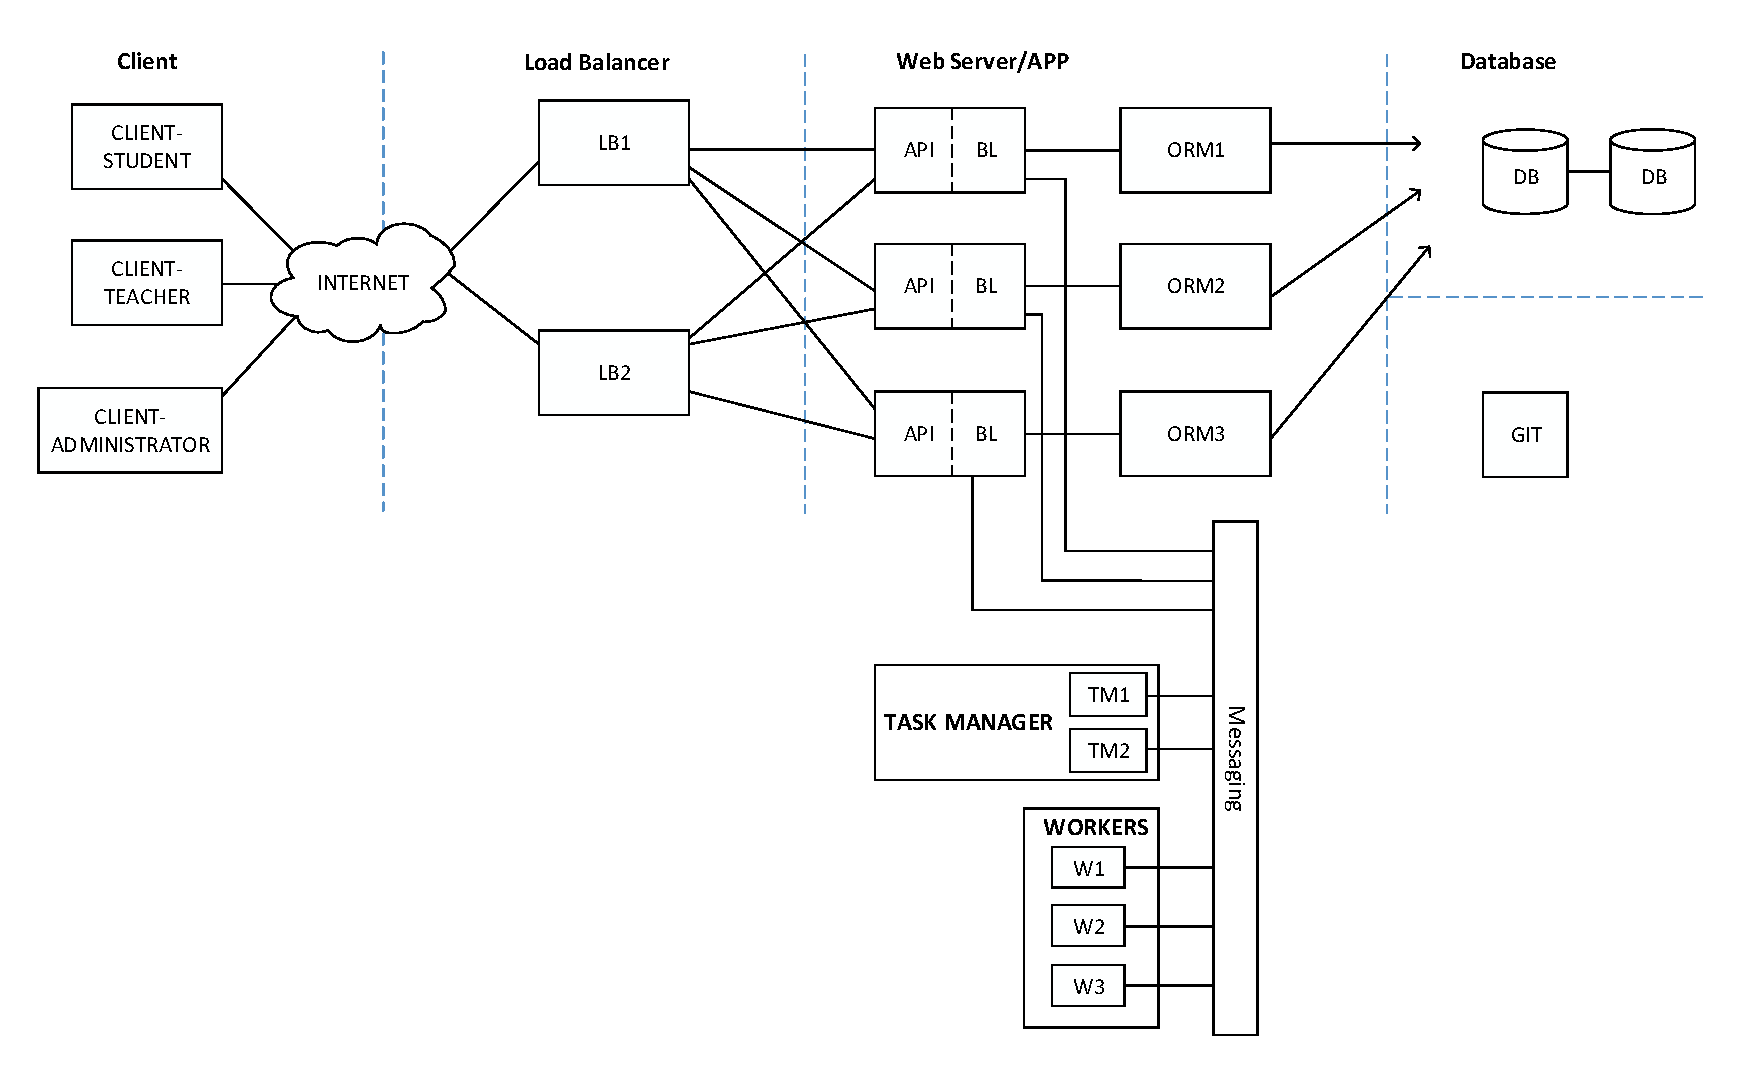
\includegraphics[height=0.95\textwidth]{figures/atfogo_rendszerterv_teljes.pdf}
		\caption[Conceptional System Design]{Conceptional System Design}
		\label{fig:conceptional-system-design}
	\end{figure}
\end{landscape}

\section{Scalability}

\newparagraph{Client}
To solve the scalability problem, the client's code will run in a web browser for every user. This way, resources for the client's code are provided by the user as he opens the web portal in a web browser.
 
\newparagraph{Web Server}
If there were not any load balancer between the client and the web server, then one server would get every request. With thousands of users this could lead to overload and high the response time. With a load balancer, the requests will first arrive at the load balancer, and it will decide which web server will handle that request and forwards it to that web server. The choice depends on the client module, request type and the web servers' load. The load balancer's purpose is to avoid overload and minimize the response time.


 
 \section{Data Security}
 Both the back end and the front end are divided into three big modules: student, teacher and administrator. 

 \newparagraph{Web Server}
 This gives us the option to run the different modules on different computers or virtual machine instances.
 
 \newparagraph{Client}
 This ensures that one module's source code is not enough to deduce the available data, e.g., the student module will not include some API routing rules, that are included in the teacher module and the administrator module.
 

\section{Entity–Relationship Model}
\label{ER-model}

A data model describes the structures in which the database stores the data. The \emph{Entity-Relationship model} is a formal notation, that describes the data structure with entities and the relationships between them. An \emph{entity} is an existing information, that needs to be modeled. \emph{Properties (attributes)} describes the entities and makes them unique. A \emph{relationship} describes a connection between entities~\cite{adatb}.
 
The project's model uses Chen's notation. About 65 percent of the model was created by me, 35 percent of it was created by József Marton and it was finalized by the team. The attribute list is in \refstruc{attribute-list}.

The main entities are the followings:

\begin{itemize}
	\item \textbf{Appointments:} An appointment connects the student groups with a date and a location.
	\item \textbf{Courses:} The courses, that use the portal.
	\item \textbf{Deliverables:} The things to be submitted by the students (e.g. homework).
	\item \textbf{Deliverables/Repositories:} A special type of Deliverables that is to be submitted through a repository.
	\item \textbf{Deliverables/Files:} A special type of Deliverables that is to be submitted as a file upload.
	\item \textbf{DeliverableTypes:} Describes the type of the submitted homework, e.g. documentation, source code. 
	\item \textbf{Events:} An educational event is a class with a date for a particular student to participate.
	\item \textbf{EventTypes:} An event can be any type of class: lecture, laboratory or seminar. The Software Laboratory course has only laboratories.
	\item \textbf{ExerciseCategories:} Describes the type of the laboratory: DBMS, SQL, JDBC, XML technologies in databases or SOA.
	\item \textbf{ExerciseTypes:} Describe the topic and the language of the exercises. 
	\item \textbf{RegisteredStaffs:} A many-to-many relationship between the Semesters and the Staffs. It describes the staff member's role in the semester.
	\item \textbf{RegisteredStudents:} A many-to-many relationship between the Semesters and the Students. It describes which Neptun course the student registered for in the semester.
	\item \textbf{Semesters:} An instance of the course in a particular academic term.
	\item \textbf{StudentGroups:} In Software Laboratory 5 the students are assigned to different groups. A group has one demonstrator and about 20 students.
	\item \textbf{Users:} People, that use the portal during a semester.
	\item \textbf{Users/Staffs:} A type of user, who is not a student. This user can be an administrator and/or a demonstrator and/or an evaluator.
	\item \textbf{Users/Students:} A type of user, who attends the laboratories and solves a list of tasks.
\end{itemize}

\begin{landscape}
	
	\begin{figure}[!htbp]
		\centering
		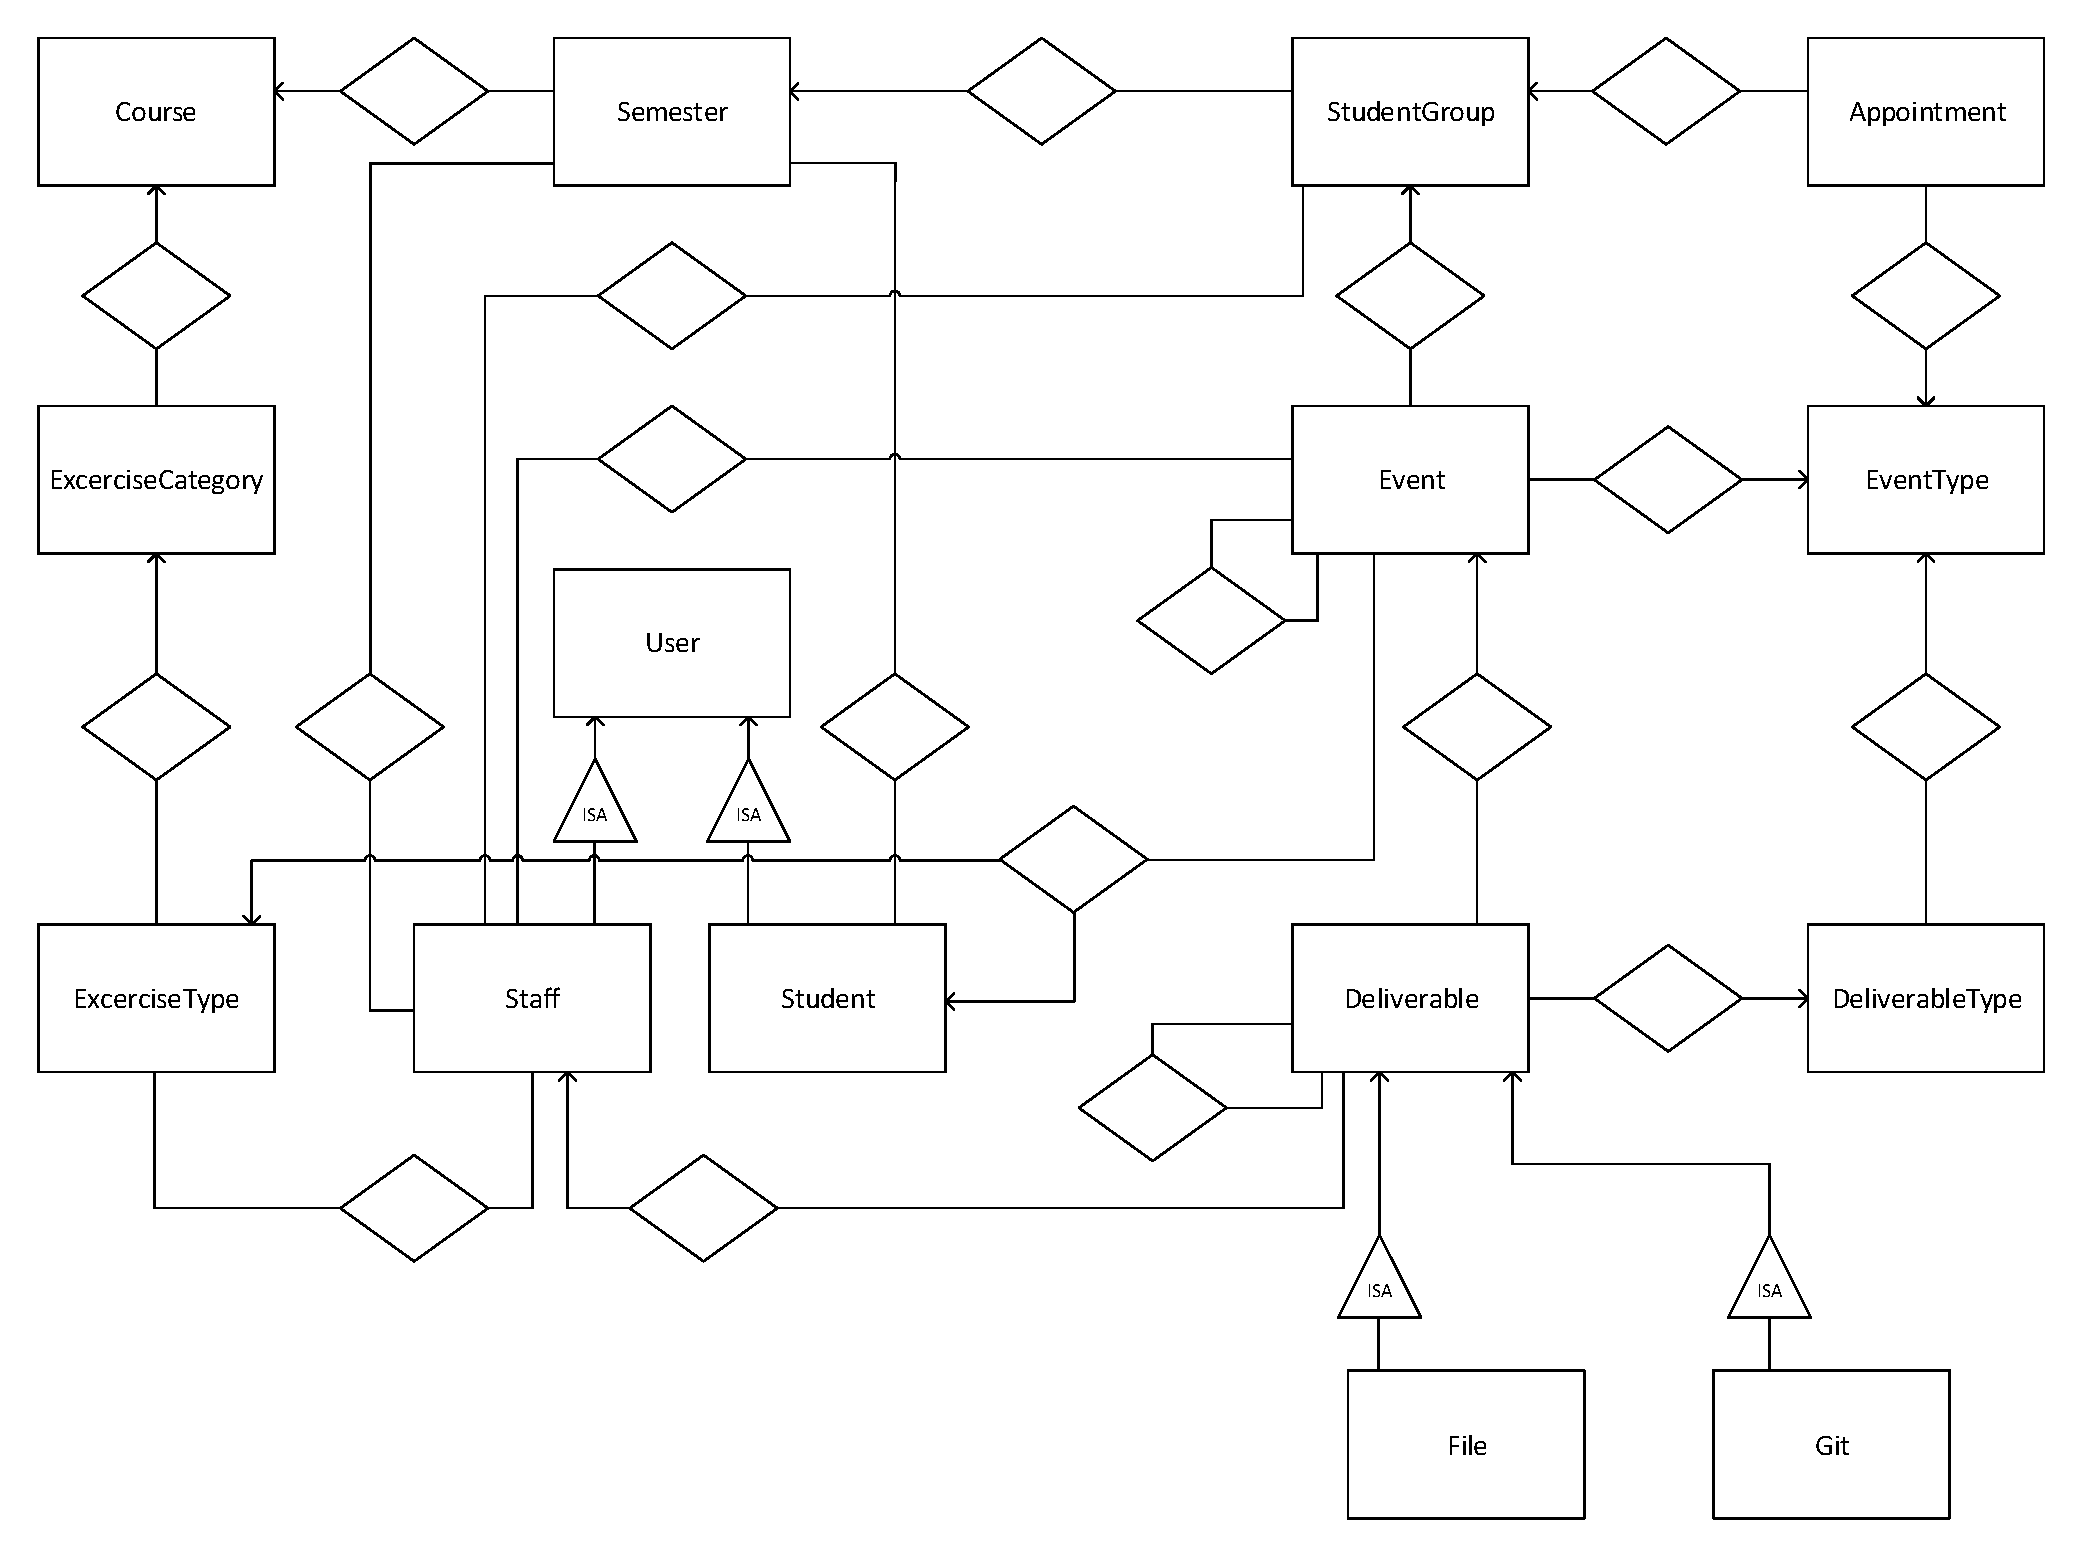
\includegraphics[width=1.3\textheight]{figures/ER.pdf}
		\caption[Entity–relationship model]{Entity–relationship model}
		\label{fig:er}
	\end{figure}
\end{landscape}



